% Provide the results in the form of Tables/Graphs
% Add a description also

\subsection{Classification Report Analysis}

The table \ref{table:classification_report} presents the classification
performance of the proposed MDIF framework across the three classes.

\begin{table}[h!t]
  \caption{Classification Report}
  \begin{center}
    \begin{tabularx}{\linewidth}{Ycccc}
      \toprule
                                &\textbf{Precision} &\textbf{Recall} &\textbf{F1-Score} &\textbf{Support} \\

      \midrule
      \textit{Authentic}        & 0.92              & 0.92           & 0.92             & 15226 \\
      \textit{Generated}        & 0.96              & 0.97           & 0.97             & 11797 \\
      \textit{Inpainted}        & 0.68              & 0.66           & 0.67             & 2494 \\
      \midrule
      \textit{Accuracy}         & --                & --             & 0.92             & 29517 \\
      \textit{Macro Average}    & 0.86              & 0.85           & 0.85             & 29517 \\
      \textit{Weighted Average} & 0.92              & 0.92           & 0.92             & 29517 \\
      \bottomrule
    \end{tabularx}
    \label{table:classification_report}
  \end{center}
\end{table}


The model achieved an overall classification accuracy of 92\%, showing a strong
general detection capability across authentic, AI-generated and AI-manipulated
images. With a precision of 0.96, a recall of 0.97 and an F1-score of 0.97, the
AI generated class achieved the highest performance, demonstrating the easily
detectable inconsistencies these images had in their spatial and spectral
domain.

The Authentic class was not too far behind with an F1 Score of 0.92, showing the
model's successful rate of classification with minimal false positives and false
negatives.

The Inpainted class achieved a lower performance in comparison, with a precision
of 0.68, recall of 0.66 and F1score of 0.67, which was expected considering how
the inpainted images contain only localized modifications with most of the image
being authentic. Detection of subtle manipulations are more difficult, however,
despite the challenge, the model achieved a meaningful detection capability due
to the inclusion of spectral inconsistency analysis, boundary artifact detection
and depth shading discrepancy analysis.

The macro average F1 Score of 0.85 is a balanced score on the performance across
all the classes. The weighted average F1 score on the other hand reached a
staggering 0.92 reflecting the model's stability despite the class imbalance.

\subsection{Confusion Matrix}

\begin{figure}
  \centering
  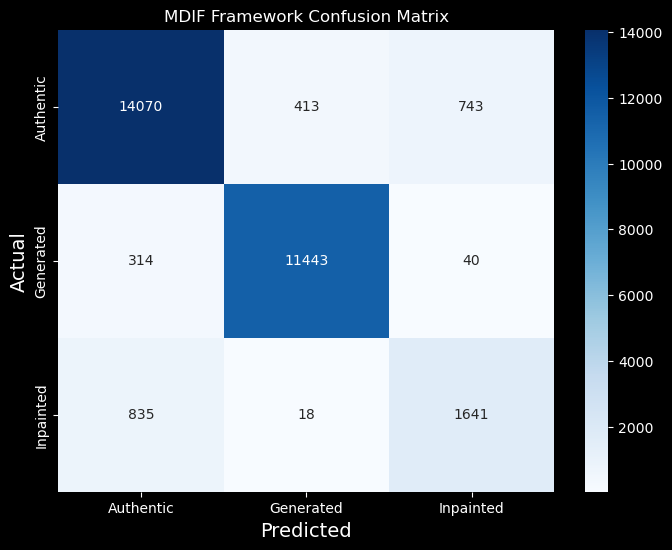
\includegraphics[width=\linewidth]{figs/conf_matrix.png}
  \caption{Confusion Matrix of the three classes: Authentic,
  Generated, and Inpainted}
  \label{fig:conf_matrix}
\end{figure}

The confusion matrix as in figure \ref{fig:conf_matrix} clearly illustrates the
detailed prediction behavior of the model, which correctly classified 14,070
authentic images, 11,443 generated images and 1,641 inpainted images. Most of
the classification errors occurred between Authentic and Inpainted classes due
to the inpainted image's preservation of most of its original authentic
structure, making the slight manipulation difficult to identify. The Generated
class displayed least confusion with other categories during identification,
confirming the strong detectable inconsistencies in these images. The confusion
matrix confirms the role of the proposed hybrid feature fusion strategy in
separating the three classes precisely while maintaining a reasonable detection
capability for localized manipulations.

\subsection{ROC Curve Analysis}

\begin{figure}
  \centering
  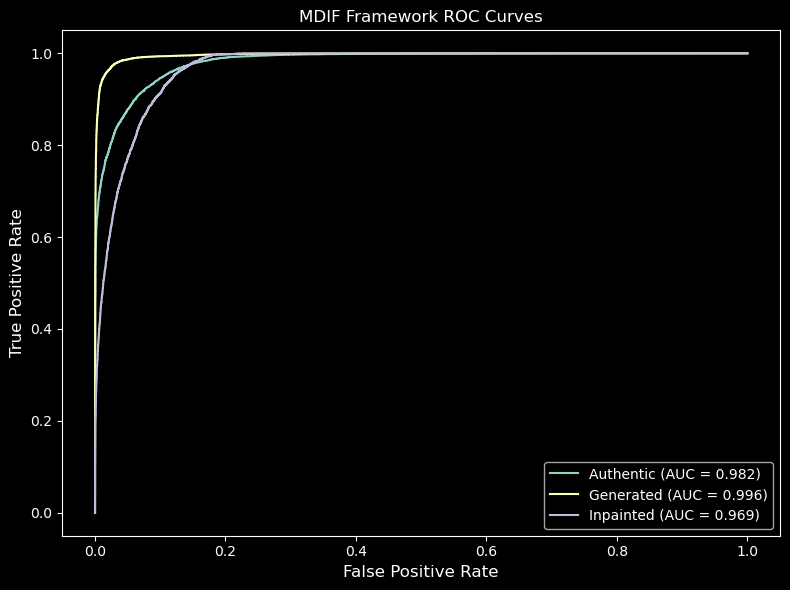
\includegraphics[width=\linewidth]{figs/roc_curves.png}
  \caption{ROC Curves for the three classes: Authentic, Generated,
  and Inpainted}
  \label{fig:roc_curves}
\end{figure}

The ROC curve displayed in figure \ref{fig:roc_curves} shows the results of the
model's clear ability to distinguish the classes in the framework with the AUC
values of 0.982, 0.996 and 0.969 for Authentic, Generated and Inpainted classes
respectively. The Generated class's near-perfect discrimination is all because
of the strong spectral and texture inconsistencies displayed by AI-generated
images. Although the Inpainted class achieved a slightly slower performance, its
AUC value indicates a very strong detection capability for the localized
manipulations.

\subsection{Precision-Recall Curve Analysis}

\begin{figure}
  \centering
  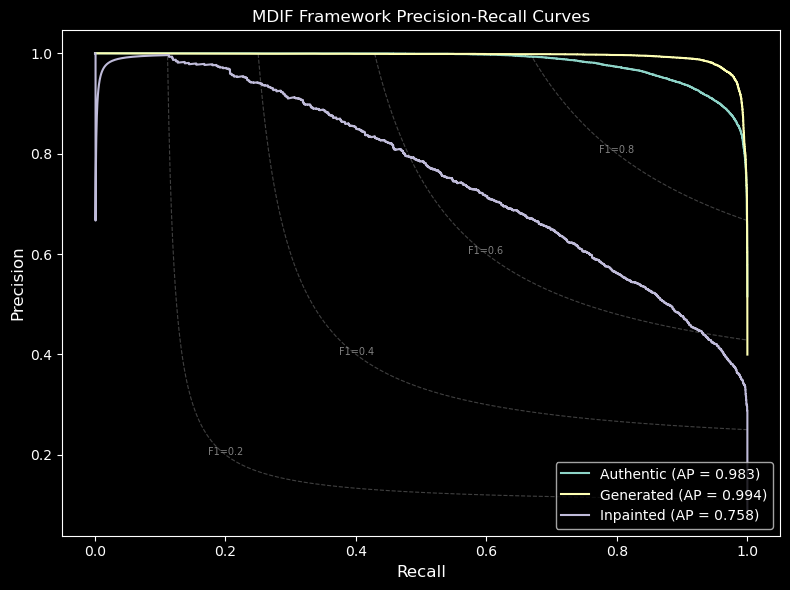
\includegraphics[width=\linewidth]{figs/pr_curves.png}
  \caption{Precision-Recall Curves for the three classes: Authentic, Generated,
  and Inpainted}
  \label{fig:pr_curves}
\end{figure}

The Precision-Recall curves as seen in figure \ref{fig:pr_curves} further
validate the model's efficiency under class imbalance conditions with the
Average Precision (AP) scores touching 0.983 for Authentic, 0.994 for Generated
and 0.758 for Inpainted classes. The high AP scores for Authentic and Generated
classes are a testimony to their stable precision across varying recall
thresholds. The difficulty in detection of local manipulation is precisely why
the Inpainted class achieved a lower AP score, although it is acceptable
considering the complexity of Inpainting detection. These results validate the
combination strategy applied in the model with the spatial, spectral and depth
domain inconsistencies' tendency to improve model durability against synthetic
and partially synthetic images.
